\documentclass[10pt]{article}

\usepackage{xspace}
\usepackage{amsmath,amssymb}
\usepackage{adjustbox}
\usepackage[dvipsnames]{xcolor}
\usepackage{multirow}
\usepackage{datetime}
\usepackage{caption}

%% Use these lines for letter-sized paper
\usepackage[paper=letterpaper,
%%             nofoot, % Uncomment to put page number above margin
%%             marginparwidth=1in,     % Length of section titles
%%             marginparsep=.05in,       % Space between titles and text
               margin=1in,               % 1 inch margins
            left=1.0in,
            right=1.0in,
%%             includemp
            ]{geometry}

%% More layout: Get rid of indenting throughout entire document
\setlength{\parindent}{0in}

\begin{document}
\thispagestyle{empty}

\today, \currenttime


\section{Layout of the Endcap Petal}

Figure~\ref{endcap_model} depicts the endcap petal model used for calculating thermal impedances.

\begin{figure}[ht!]
\begin{center}
\includegraphics[width=0.99\linewidth]{figures/m30C_0Wm2C_Setup_BPOL12V.pdf}
\end{center}
\caption{The endcap petal model used for extracting thermal impedances. The front-end components are
labeled in R0 (the rightmost module).}
\label{endcap_model}
\end{figure}

The number of BPOL12Vs, AMACs, ABCs, HCC, and the sensor area of each module are listed in
Table~\ref{tab:layout_parameters}.
%
\let\arraystretcha\arraystretch
\renewcommand\arraystretch{1.1} % 1.6
\begin{table}[h]
\begin{center}
\adjustbox{max width=\textwidth}{ %% just before tabular
\begin{tabular}{|l|r|r|r|r|r|r|} \hline
Module & nBPOL12V & nAMAC & nABC & nHCC & Sensor area (cm$^2$) \\ \hline
R0     &      1 &     1 &   17 &    2 &                 92.0 \\
R1     &      1 &     1 &   21 &    2 &                 91.0 \\
R2     &      1 &     1 &   12 &    2 &                 76.0 \\
R3     &      2 &     2 &   28 &    4 &                164.0 \\
R4     &      1 &     1 &   16 &    2 &                178.0 \\
R5     &      1 &     1 &   18 &    2 &                186.0 \\
\hline \end{tabular}
} %% resizebox after tabular
\end{center}
\caption{Number of components on each module.}
\label{tab:layout_parameters}
\end{table}
\let\arraystretch\arraystretcha


\clearpage

\clearpage

\newcommand{\highlight}[1]{{\color{BrickRed}\textbf{#1}}}

\section{Power Inputs for the Endcap Petal Model}

Table~\ref{tab:power_numbers} details the current, voltage, and power specifications for each
front-end component. The values should match the numbers used in the barrel thermal model.

\def\tid{\ensuremath{^*\xspace}}
\def\eff{\ensuremath{\varepsilon}}
\def\pfeast{\ensuremath{\frac{(1-\eff)}{\eff}(P_\text{ABC}+P_\text{HCC})}}
%
\let\arraystretcha\arraystretch
\renewcommand\arraystretch{1.2} % 1.6
\begin{table}[h!]
\begin{center}
\adjustbox{max width=\textwidth}{ %% just before tabular
\begin{tabular}{|l|c|c|c|c|c|c|c|} \hline
\multirow{2}{*}{Description} & input voltage & \multicolumn{4}{c|}{Specifications for 1 component} & $n$ components & Total power \\
              & [V]           & current [A] &\% bumped & power [W]                   & eff   & per module (1 side) & (1 side) [W] \\ \hline
AMAC 1.5V     & 1.5           & 0.042               &  & 0.063                       &       & --                  &       \\
AMAC 2.5V     & 2.5           & 0.002               &  & 0.005                       &       & --                  &       \\
Total AMAC    & --            & --                  &  & \color{blue}{0.068}         &       & R3: 2               & 0.136 \\
              &               &                     &  &                             &       & All others: 1       & 0.068 \\ \hline
ABC (digital) & 1.5           & 0.027          & 110\% & 0.0405                      &       & --                  &       \\
ABC (analog)  & 1.5           & 0.068               &  & 0.102                       &       & --                  &       \\
Total ABC     & --            & 0.095               &  & \color{blue}{0.1425}\tid    &       & R0: 17              & 2.423 \\
              &               &                     &  &                             &       & R1: 21              & 2.993 \\
              &               &                     &  &                             &       & R2: 12              & 1.710 \\
              &               &                     &  &                             &       & R3: 28              & 3.990 \\
              &               &                     &  &                             &       & R4: 16              & 2.280 \\
              &               &                     &  &                             &       & R5: 18              & 2.565 \\ \hline
HCC (digital) & 1.5           & 0.210         & 25.5\% & 0.315                       &       & --                  &       \\
HCC (analog)  & 1.5           & 0.0                 &  & 0.0                         &       & --                  &       \\
Total HCC     & --            & 0.210               &  & \color{blue}{0.315}\tid     &       & R3: 4               & 1.260 \\
              &               &                     &  &                             &       & All others: 2       & 0.630 \\ \hline
bPOL12V (ABC,HCC,AMAC1.5) & --&                     &  & \pfeast   \tid              & 72\%  & --                  & R0: \color{blue}{1.187} \\
              &               &                     &  &                             &       &                     & R1: \color{blue}{1.409} \\
              &               &                     &  &                             &       &                     & R2: \color{blue}{0.910} \\
              &               &                     &  &                             &       &                     & R3: \color{blue}{1.021+1.021} \\
              &               &                     &  &                             &       &                     & R4: \color{blue}{1.132} \\
              &               &                     &  &                             &       &                     & R5: \color{blue}{1.243} \\ \hline
linPOL12V (for AMAC2.5) & --  &                     &  & see text                    &       & --                  & R3: \color{blue}{0.450 + 0.450} \\
              &               &                     &  &                             &       & --                  & All others: \color{blue}{0.450} \\ \hline
Total Module  & --            &                     &  & \tid                        &       &                     & R0: 4.758 \\
              &               &                     &  &                             &       &                     & R1: 5.549 \\
              &               &                     &  &                             &       &                     & R2: 3.768 \\
              &               &                     &  &                             &       &                     & R3: 8.328 \\
              &               &                     &  &                             &       &                     & R4: 4.560 \\
              &               &                     &  &                             &       &                     & R5: 4.956 \\ \hline
\multicolumn{8}{|c|}{} \\[-2mm]
\multicolumn{8}{|c|}{EOS} \\ \hline
lpGBT                     & 1.2         & 0.317     &  & 0.380                       &       & --                  & \color{blue}{0.380} \\ \hline
VTRx (VL+) GBLD 1.2V      & 1.2         & 0.025     &  & 0.030                       &       & --                  & \\
VTRx (VL+) GBLD 2.5V      & 2.5         & 0.07      &  & 0.175                       &       & --                  & \\
VTRx (VL+) GBTIA (legacy) & 2.5         & 0.053     &  & 0.133                       &       & 1                   & \\
Total VTRx (VL+)          &             &           &  & 0.338                       &       & 1                   & \color{blue}{0.338} \\ \hline
bPOL2V5 (old DCDC2)       &             &           &  &                             & 88\%  & 2$\times$, master only         & \color{blue}{0.056+0.056} \\
bPOL12V       &               &                     &  &                             & 55\%  & 2$\times$, master only         & \color{blue}{0.633+0.633} \\ \hline
EOS Master    &               &                     &  &                             &       &                     & 2.096 \\
EOS Slave     &               &                     &  &                             &       &                     & 0.718 \\
EOS both sides&               &                     &  &                             &       &                     & 2.814 \\
\hline \end{tabular}
} %% resizebox after tabular
\end{center}
\caption{Endcap module inputs.
Values with \tid~next to them are affected by the TID bump in one way or another. The bPOL12V efficiency
is representative only; in reality it is temperature- and current-dependent.
Note that there are two bPOL12V converters and two linPOL12V converters on R3.
Further notes are
described in the text.
}
\label{tab:power_numbers}
\end{table}
\let\arraystretch\arraystretcha

Some notes on the numbers in the table:
\begin{itemize}
\item HCC and ABC power numbers correspond to unirradiated values.
\item Items marked with a ``\tid'' are affected by the digital current increase caused by the TID.
The bPOL12V is affected by the TID bump insofar as its power is determined by the ABC and HCC.
%% \item In the ABC, we have 42.5~mA digital with a 69\% bump, plus 70~mA analog. This is equivalent to
%% 29~mA fully bumped, and 83~mA non-bumped current. (Old values.)
\item The HCC is assumed to have a smaller TID bump than the ABC. This is accounted by an additional
scaling for the HCC case - see Section~\ref{tid_parameterization_details}. But because this scaling
is functionally the same as the ABC bump fraction, we write it here as well.
\item In the above, the bPOL12V efficiency is assumed to be constant, but in reality it is temperature- and
current-dependent.
\item In the EOS, the bPOL12V has a lower efficiency than in the module because the current load is
much smaller, and the bPOL12V is much less efficient in this regime.
\item The total module power (before irradiation, before TID bump) in the table represents
all components excluding HV and tape losses, which are small in comparison.
\end{itemize}

\noindent
Comments on the EOS components:

\begin{itemize}
%% \item For the EOS, the total power for both sides is simply double the power of one side.
\item The EOS bPOL12Vs and bPOL2V5s (was DCDC2) exist on one side only, and power the EOS cards on both petal
sides. There are two of each (one per side). Therefore the EOS numbers are split into ``master'' and ``slave'' numbers.
%% \item For $n=1$ lpGBTx ASICs (corresponding to the barrel long strips and the endcaps),
%% and assuming a BPOL12V efficiency $\varepsilon_\text{BPOL12V}=0.75$,
%% the total power is 1.4~W per EOS side.
%% \item For $n=2$ lpGBTx ASICs (corresponding to the barrel short strips), the total power is 2.6~W per
%% EOS side.
\end{itemize}

%% \subsection{The End-of-Substructure (EOS)}
%% \begin{itemize}
%% \item DCDC2 converter: $P=0.208$~W (see calculation below)
%% \item BPOL12V: $P=1.12$~W (see calculation below)
%% \item VTRx
%%   \begin{itemize}
%%     \item GBTIA: $I=53$~mA; 2.5~V; $P=0.1325$~W
%%     \item GBLD$_{2.5V}$: $I=18$~mA 2.5~V; $P=0.045$~W
%%   \end{itemize}
%% \item lpGBTx: $I=625$~mA; 1.2~V; $P=0.75$~W; powered by DCDC2
%% \item GBLD$_{1.2V}$: $I=9.5$~mA; 1.2~V; $P=0.0114$~W; powered by DCDC2
%% \end{itemize}

\subsection{Power Equations for the EOS, bPOL12V, bPOL2V5 and linPOL12V}

The total power of the EOS (one side) is given by:
\begin{equation}
P_\text{EOS} = \frac{1}{\varepsilon_\text{bPOL12V}}\times
  \left( \frac{1}{\varepsilon_\text{bPOL2V5}} (n P_\text{lpGBTx} + n P_\text{GBLD1.2}) + n P_\text{GBLD2.5} + P_\text{GBTIA} \right)
\end{equation}
% (((.750*2+0.0114*2)/0.88)+0.1325+0.045*2)/0.75 = 2.60
% (((.750*1+0.0114*1)/0.88)+0.1325+0.045*1)/0.75 = 1.40

As can probably be inferred from above, the power attributed to the EOS bPOL12V is:
\begin{equation}
P^\text{EOS}_\text{bPOL12V} = \frac{(1-\varepsilon_\text{bPOL12V})}{\varepsilon_\text{bPOL12V}}\times
  \left( \frac{1}{\varepsilon_\text{bPOL2V5}} (n P_\text{lpGBTx} + n P_\text{GBLD1.2}) + n P_\text{GBLD2.5} + P_\text{GBTIA} \right)
\end{equation}

The power in the EOS bPOL2V5 (was called DCDC2) converter is:
\begin{equation}
P^\text{EOS}_\text{bPOL2V5} = \frac{(1-\varepsilon_\text{bPOL2V5})}{\varepsilon_\text{bPOL2V5}} \left(n P_\text{lpGBTx} + n P_\text{GBLD1.2}\right)
\end{equation}


The power dissipated by the linPOL12V (powering the AMAC) is given by the current in the AMAC components
(adding the quiescent current, 1.9 mA) multiplied by the voltage drop in the linPOL12V:
\begin{equation}
P_\text{linPOL12V} = (I^{1.5V}_\text{AMAC} + I^\text{q}_\text{linPOL12V})\left(  \Delta V_\text{linPOL12V} - 1.5V \right)
                   + (I^{3.0V}_\text{AMAC} + I^\text{q}_\text{linPOL12V})\left(  \Delta V_\text{linPOL12V} - 3.0V \right)
\label{eq:amac_regulator}
\end{equation}
where the calculation of $\Delta V_\text{linPOL12V}$ is described in Section~\ref{low_voltage}.

\subsection{bPOL12V (FEAST) efficiency}

The bPOL12V efficiency varies as a function of temperature and load current. The parameterization used
is the one derived by Georg. Figure~\ref{feast_vs_temperature} highlights the agreement between the
measured FEAST efficiencies and the parameterized fit.

\begin{figure}[ht!]
\begin{center}
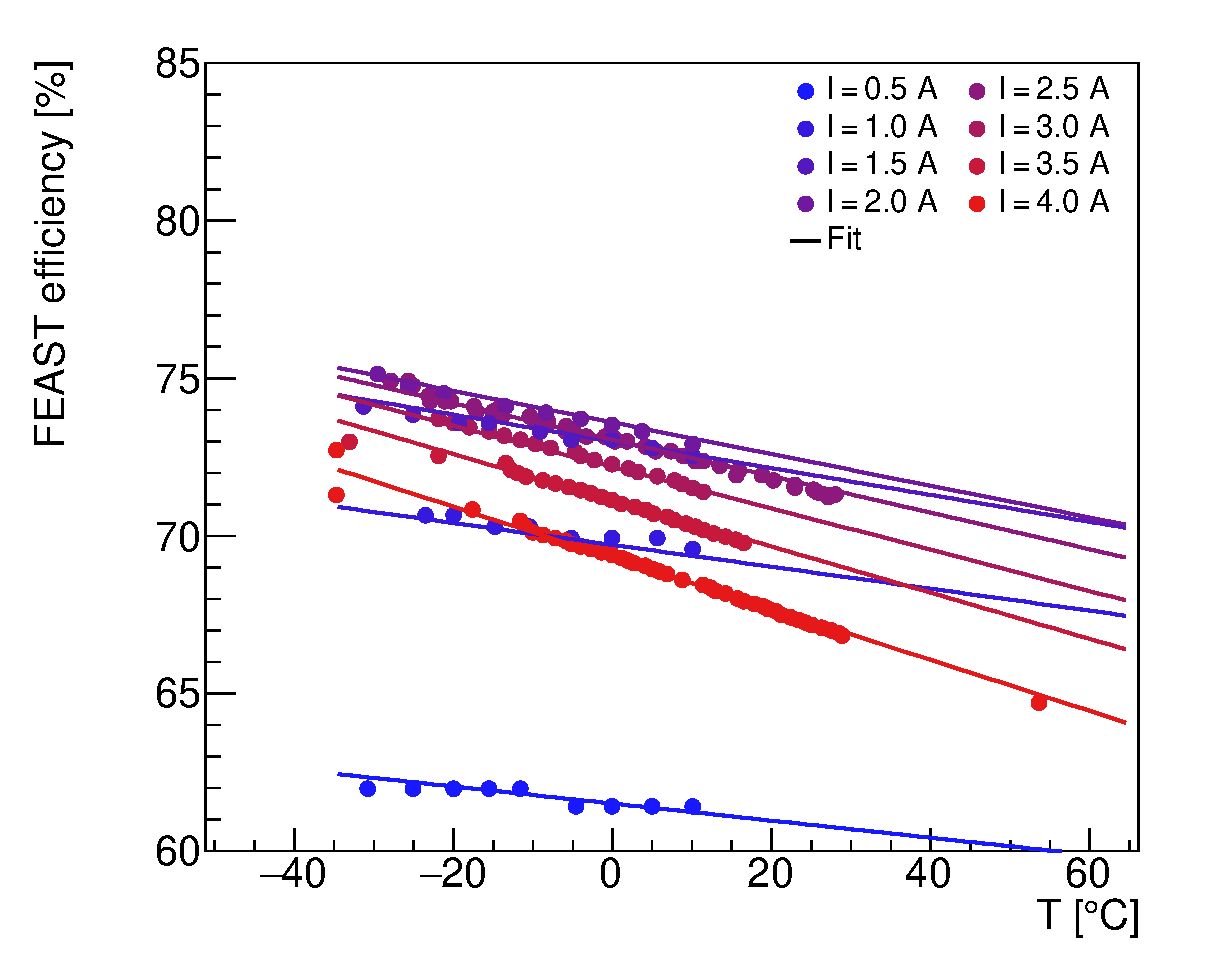
\includegraphics[width=0.49\linewidth]{figures/FeastEfficiency_isoCurrent}
\end{center}
\caption{FEAST efficiency data versus temperature ($x$-axis) and current (indicated with different
colors). The parameterization of the data is represented by the fit lines at fixed current.
}
\label{feast_vs_temperature}
\end{figure}

\subsection{TID bump parameterization}
\label{tid_parameterization_details}

The TID bump parameterization is the one supplied by Kyle Cormier for the ABC130$^{*}$
(Nominal parameters: $a=1.402\times 10^{11}$, $b=-1.62$.
Pessimistic parameters: $a=2.64\times10^{9}$, $b=-1.35$.)
Figure~\ref{tid_parameterization} shows the TID parameterization used in the current model. This
parameterized bump is applied to the ``bumped'' fraction of digital current, as indicated in
Table~\ref{tab:power_numbers}.

\begin{figure}[ht!]
\begin{center}
\begin{subfigure}[t]{0.49\textwidth}\includegraphics[width=0.99\linewidth]{figures/AbcTidBumpVersionRatesAndTemps_Nominal}\caption{Nominal Case}\end{subfigure}
\begin{subfigure}[t]{0.49\textwidth}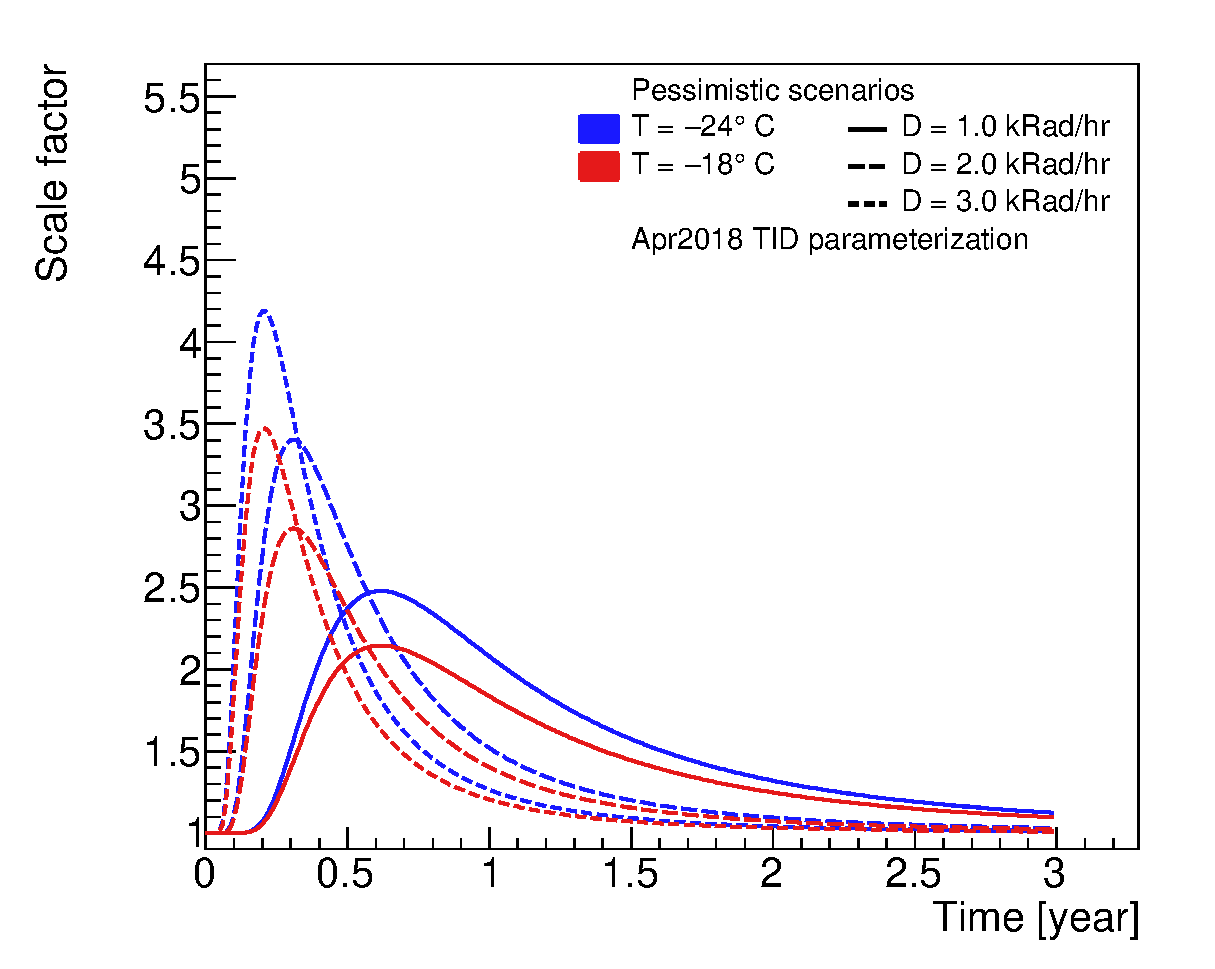
\includegraphics[width=0.99\linewidth]{figures/AbcTidBumpVersionRatesAndTemps_Pessimistic}\caption{Pessimistic Case}\end{subfigure}
\end{center}
\caption{TID parameterization vs time, for two representative temperatures (indicated by
color) and three dose rates (indicated by line style). Nominal and Pessimistic cases are shown.}
\label{tid_parameterization}
\end{figure}

\subsubsection*{HCC Treatment}

The HCC is assumed to have a smaller TID bump than the ABC. Thus, the HCC TID bump
is scaled by a factor (see Table~\ref{tab:power_numbers}) to account for the smaller observed HCC TID bump.

\subsection{Summary of Power Contributions in R1}

A stack plot showing the contributions of each component to the total power is shown in
Figure~\ref{power_stackplot}.

\begin{figure}[ht!]
\begin{center}
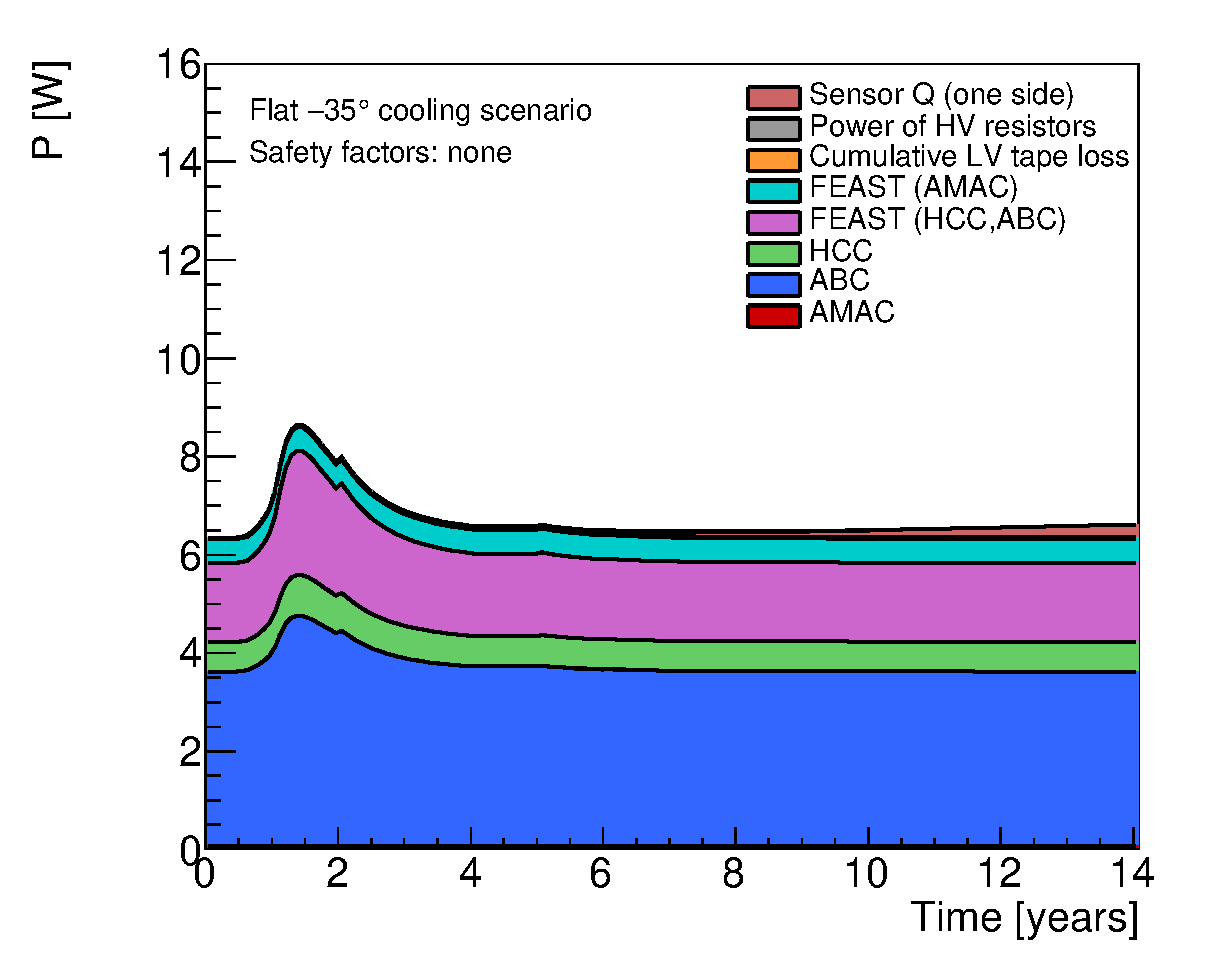
\includegraphics[width=0.55\linewidth]{figures/PowerStackPlot.eps}
\end{center}
\caption{Summary of the contributions of each front-end component to the total power in R3 (Disk 5), given
a nominal TID bump parameterization and no safety factors, to illustrate the relative contributions
of each component.}
\label{power_stackplot}
\end{figure}


\clearpage

\newcommand{\highlight}[1]{{\color{BrickRed}\textbf{#1}}}

\section{Collecting Power Inputs for the Endcap Petal}

Table~\ref{tab:power_numbers} details the current, voltage, and power specifications for each
component. Most of these numbers come from Graham and Georg's thermal model. Most are similar to
Sergio's numbers, with some differences highlighted in red.

\def\tid{\ensuremath{^\text{TID}}\xspace}
\def\eff{\ensuremath{\varepsilon}}
\def\pfeast{\ensuremath{\frac{(1-\eff)}{\eff}(P_\text{ABC}+P_\text{HCC})}}
%
\let\arraystretcha\arraystretch
\renewcommand\arraystretch{1.2} % 1.6
\begin{table}[h]
\begin{center}
\adjustbox{max width=\textwidth}{ %% just before tabular
\begin{tabular}{|l|c|c|c|c|c|c|} \hline
\multirow{2}{*}{Description} & input voltage & \multicolumn{3}{c|}{Specifications for 1 component} & $n$ components & Total power \\
              & [V]           & current [A]           & power [W]                   & eff   & per module (1 side) & (1 side) [W]    \\ \hline
AMAC 1.5V     & 1.5           & 0.045                 & 0.0675                      &       & --                  &                 \\
AMAC 3.0V     & 3.0           & 0.002                 & 0.006                       &       & --                  &                 \\
Total AMAC    & --            & --                    & 0.0735                      &       & 1                   & 0.0735          \\ \hline
ABC (digital) & 1.5           & 0.035                 & 0.0525                      &       & --                  &                 \\
ABC (analog)  & 1.5           & 0.066                 & 0.099                       &       & --                  &                 \\
Total ABC     & --            & 0.101                 & 0.1515                      &       & 21$^*$              & 3.1815$^*$\tid  \\ \hline
HCC (digital) & 1.5           & 0.125                 & 0.1875                      &       & --                  &                 \\
HCC (analog)  & 1.5           & 0.075                 & 0.1125                      &       & --                  &                 \\
Total HCC     & --            & 0.200                 & 0.3                         &       & 2$^*$               & 0.6$^*$\tid     \\ \hline
FEAST (ABC,HCC) & --          &                       & \pfeast                     & 75\%  & --                  & 1.2605$^*$\tid  \\
``FEAST'' AMAC regulators & --&                       & see below                   &       & --                  & 0.415           \\
Total FEAST   & --            &                       & see below                   &       & 1                   & 1.6755$^*$\tid  \\ \hline
Total Module (R1)  & --       &                       &                             &       &                     & 5.53$^*$        \\ \hline
\multicolumn{7}{|c|}{} \\[-2mm]
\multicolumn{7}{|c|}{EOS} \\ \hline
VTRx: lpGBTx  & 1.2           & 0.625                 & 0.750                       &       & --                  &                 \\
VTRx: GBLD 1.2V & 1.2         & 0.0095                & 0.0114                      &       & --                  &                 \\
VTRx: GBLD 2.5V & 2.5         & 0.018                 & 0.045                       &       & --                  &                 \\
Total VTRx    &               &                       & 0.8064                      &       & 1                   & 0.8064          \\         
GBTIA         & 2.5           & 0.053                 & 0.1325                      &       & 1                   & 0.1325          \\
FEAST         &               &                       &                             &       & 0.5$^\dagger$       & 0.35$^\dagger$  \\
DCDC2         &               &                       &                             & 88\%  & 0.5$^\dagger$       & 0.104$^\dagger$ \\ \hline
Total EOS     &               &                       &                             &       &                     & 1.4             \\
EOS both sides&               &                       &                             &       &                     & 2.8             \\
\hline \end{tabular}
} %% resizebox after tabular
\end{center}
\caption{Endcap module inputs. Starred ($^*$) values are representative and taken from Endcap R1. Values
with \tid next to them are affected by the TID bump in one way or another. The 75\% FEAST efficiency 
is representative only; in reality it is temperature- and current-dependent (also TID-dependent?).
}
\label{tab:power_numbers}
\end{table}
\let\arraystretch\arraystretcha

Some notes on the numbers in the table:
\begin{itemize}
\item HCC and ABC power numbers correspond to unirradiated values.
\item The ABC power numbers (from Georg/Graham) differ from Sergio's sheet by 1.7\%.
\item \highlight{The HCC power numbers (from Georg/Graham) differ from Sergio's sheet by 38\%.}
\item \tid The FEAST is affected by the TID bump insofar as its power is determined by the ABC and HCC.
  In the above it is assumed to be 75\%, but it is temperature and current-dependent.
\item The total power (before irradiation, before TID bump) of Module R1 represents
all components excluding HV and tape losses, which are small in comparison.
\item For the EOS, the total power for both sides is simply double the power of one side.
\item $^\dagger$ The FEAST and DCDC2 exist on one side only, and power the EOS cards on both petal
sides (hence ``0.5 per side''). If both EOSes are powered, then the power dissipatd by the FEAST and
DCDC2 is twice the power listed above.
\item For $n=1$ lpGBTx ASICs (corresponding to the barrel long strips and the endcaps),
and assuming a FEAST efficiency $\varepsilon_\text{FEAST}=0.75$,
the total power is 1.4~W per EOS side.
\item For $n=2$ lpGBTx ASICs (corresponding to the barrel short strips),
\highlight{the total power is 2.6~W per EOS side (differs from the TDR, which says 3~W)}.
\end{itemize}

%% \subsection{The End-of-Substructure (EOS)}
%% \begin{itemize}
%% \item DCDC2 converter: $P=0.208$~W (see calculation below)
%% \item FEAST: $P=1.12$~W (see calculation below)
%% \item VTRx
%%   \begin{itemize}
%%     \item GBTIA: $I=53$~mA; 2.5~V; $P=0.1325$~W
%%     \item GBLD$_{2.5V}$: $I=18$~mA 2.5~V; $P=0.045$~W
%%   \end{itemize}
%% \item lpGBTx: $I=625$~mA; 1.2~V; $P=0.75$~W; powered by DCDC2
%% \item GBLD$_{1.2V}$: $I=9.5$~mA; 1.2~V; $P=0.0114$~W; powered by DCDC2
%% \end{itemize}

The total power of the EOS (one side) is given by:
\begin{equation}
P_\text{EOS} = \frac{1}{\varepsilon_\text{FEAST}}\times
  \left( \frac{1}{\varepsilon_\text{DCDC2}} (n P_\text{lpGBTx} + n P_\text{GBLD1.2}) + n P_\text{GBLD2.5} + P_\text{GBTIA} \right)
\end{equation}
% (((.750*2+0.0114*2)/0.88)+0.1325+0.045*2)/0.75 = 2.60
% (((.750*1+0.0114*1)/0.88)+0.1325+0.045*1)/0.75 = 1.40

As can probably be inferred from above, the power in the EOS FEAST is:
\begin{equation}
P^\text{EOS}_\text{FEAST} = \frac{(1-\varepsilon_\text{FEAST})}{\varepsilon_\text{FEAST}}\times
  \left( \frac{1}{\varepsilon_\text{DCDC2}} (n P_\text{lpGBTx} + n P_\text{GBLD1.2}) + n P_\text{GBLD2.5} + P_\text{GBTIA} \right)
\end{equation}

The power in the EOS DCDC2 converter is:
\begin{equation}
P^\text{EOS}_\text{DCDC2} = \frac{(1-\varepsilon_\text{DCDC2})}{\varepsilon_\text{DCDC2}} \left(n P_\text{lpGBTx} + n P_\text{GBLD1.2}\right)
\end{equation}


The power dissipated by the AMAC regulators is given by the current in the AMAC components multiplied
by the voltage drop in the regulators:
\begin{equation}
P_\text{regulator} = I^{1.5V}_\text{AMAC}\left(  10.5V - 1.5V \right)
                   + I^{3.0V}_\text{AMAC}\left(  10.5V - 3.0V \right)
\label{eq:amac_regulator}
\end{equation}



\section{ Extracting thermal impedances using FEA simulations}

\subsection{Setup of the FEA Simulation to extract thermal impedances}

Representative power numbers are used to power each component. In each simulation run, all instances
of one type of component (e.g. the ABCs) are powered on in all six modules, keeping the rest off.
Average temperatures are measured for the following components (see below): HCC, ABC, FEAST, sensor.

\def\thcc{\ensuremath{\overline{T}_\text{nHCC}}}
\def\tabc{\ensuremath{\overline{T}_\text{nABC}}}
\def\tfeast{\ensuremath{\overline{T}_\text{FEAST}}}
\def\tsensor{\ensuremath{T_\text{sensor}}}
\def\Rm{\ensuremath{{\text{R}m}}}

\begin{itemize}
\item FEAST: a $3\times3$~mm $\times~350~\mu$m chip inside the shield box.
  \begin{itemize}
  \item The FEAST has an additional power term due to regulators for the AMAC -- see below.
  \end{itemize}
\item AMAC: a $3\times3$~mm $\times~350~\mu$m chip, roughly in the center of the power board
  \begin{itemize}
    \item The AMAC is powered using regulators located in the FEAST chip, with a power dissipation
      of the regulators corresponding to the voltage drop in the regulator (0.415~W) -- see Eq.~\ref{eq:amac_regulator}.
  \end{itemize}
\item HVMUX: Ignore for now
\item EOS (\highlight{3.20~W total, including both sides -- see Table~\ref{tab:power_numbers}.}) % (\highlight{3.03~W total, for both sides}):
  \begin{itemize}
  \item \highlight{Placement of these EOS power sources: ???}
%%     \item 1 lpGBT per side (\highlight{0.750~W $\times$ 2 sides})
%%     \item ``Rest'' (1 VTRX optical link per side?) (\highlight{.185~W $\times$ 2 sides}) ???
%%     \item FEAST on a single side (\highlight{1.12~W})
%%     \item DCDC2 converter on a single side (\highlight{0.21~W})
  \end{itemize}
\item Cooling: Constant 8000~W/m$^{2}$K, $-30$~C, no convection
\end{itemize}




\subsection{FEA Simulation Runs to extract thermal impedances}

For the extraction of the thermal impedances, a simplified set of input power parameters are used,
summarized in Table~\ref{tab:simulation_runs}.
In the FEA, the power is distributed over all 6 surfaces (\highlight{different from barrel treatment}).

\let\arraystretcha\arraystretch
\renewcommand\arraystretch{1.4} % 1.6
\begin{table}[h!]
\footnotesize
\begin{center}
\adjustbox{max width=\textwidth}{ %% just before tabular
\begin{tabular}{|l|l|l|l|} \hline
Simulation \# & Description                        & Input parameters           \\ \hline
1             & All HCCs powered on, rest off      & $P_\text{HCC}=0.413$~W     \\
2             & All ABCs powered on, rest off      & $P_\text{ABC}=0.149$~W     \\
3             & All FEASTs powered on, rest off    & $P_\text{FEAST}=1.5$~W$^*$ \\ \hline
\multicolumn{3}{|c|}{Extended simulations} \\ \hline
4             & Tape ``powered'' on, rest off      & skip for now \\
5             & HVMUX powered on, rest off         & skip for now \\
6             & R$_\text{HV}$ powered on, rest off & skip for now \\
7             & EOS                                & skip for now \\ % $P_\text{EOS}=3.03$~W$^{**}$
\hline \end{tabular}
} %% resizebox after tabular
\end{center}
\caption{ Description of the 7 thermal simulations required to obtain the thermal impedances.
}
\label{tab:simulation_runs}
\end{table}
\let\arraystretch\arraystretcha

$^*$ The actual nominal power of the FEAST varies for each module; however, for the simulation to extract
the thermal impedances, the power is set to 1.5~W for all FEASTs in the petal.\\






\subsection{Measurements performed in each run}

%% For each component, the temperature measured is the average of the top surface nodes of all
%% components of a given type, in a given module.

The average, min and max temperatures are taken over the volume of the elements (\highlight{different from barrel treatment}).
There are 45 measurements per simulation run in total.

The average temperatures can be measured either \highlight{on one side of the petal, or as the average of components on both sides 
of the petal}.

\begin{itemize}
\item $(\thcc)_\Rm$: The average HCC temperature of the $n$ HCCs in the module, for each module R$m$ (R0, R1, ... R5) (6~total)
\item $(\tabc)_\Rm$: The average ABC temperature of the $n$ ABCs in the module, for each module R$m$ (6~total)
\item $(\tfeast)_\Rm$: The temperature of the FEAST in the module, for each module R$n$ (6~total)
\item \tsensor, taken for R0, R1, R2, R3\_left, R3\_right, R4\_left, R4\_right, R5\_left, R5\_right (9~total) (27~total measurements):
\begin{itemize}
  \item $\tsensor^\text{Avg}$: The average sensor temperature taken over the volume of the sensor
  \item $\tsensor^\text{Max}$: The maximum sensor temperature in the module, for each module
  \item $\tsensor^\text{Min}$: The minimum sensor temperature in the module, for each module
\end{itemize}
\end{itemize}




\section{The Linear Model}

\subsection{Additional parameters in the linear model}

The number of ABCs, HCC, and the sensor area are below,
as are the FEAST currents before irradiation (pre-TID bump).
%
\let\arraystretcha\arraystretch
\renewcommand\arraystretch{1.1} % 1.6
\begin{table}[h]
\footnotesize
\begin{center}
\adjustbox{max width=\textwidth}{ %% just before tabular
\begin{tabular}{|l|r|r|r|r|r|} \hline
Module & nABC & nHCC & Sensor area (cm$^2$) & $I_\text{FEAST}$ [A] & $P_\text{FEAST}$ \\ \hline
R0     &   17 &    2 &                 92.0 &              2.12 & 1.0585 \\
R1     &   21 &    2 &                 91.0 &              2.52 & 1.2605 \\
R2     &   12 &    2 &                 76.0 &              1.61 & 0.806  \\
R3     &   28 &    4 &                164.0 &              3.63 & 1.814  \\
R4     &   16 &    2 &                178.0 &              2.02 & 1.008  \\
R5     &   18 &    2 &                186.0 &              2.22 & 1.109  \\
\hline \end{tabular}
} %% resizebox after tabular
\end{center}
\caption{Endcap module inputs. The FEAST current is calculated from the HCC and ABC values in
Table~\ref{tab:power_numbers}, and given nABC and nHCC in each module. The FEAST power is calculated
assuming a 75\% efficiency, and does not include the power due to the AMAC regulators.}
\label{tab:spurious_signal_main}
\end{table}
\let\arraystretch\arraystretcha


\subsection{Other assumed quantities}

Assumed quantities are below:
\begin{itemize}
\item $R_\text{EOS}=15.0$~K/W (guessed by Georg/Graham)
\item $R_\text{sensor}=0.02$~K/W (guessed by Georg/Graham)
\item $R_\text{tape}=0.01$~K/W per module (i.e. there are 6 such resistors in the endcap) (worst-case number)
%% \item EOS DCDC2 efficiency: 0.88
%% \item $V_\text{hybrid}=1.5$~V
%% \item $I^\text{digital}_\text{HCC}=0.125$~A (before TID damage; TID-dependent)
%% \item $I^\text{analog}_\text{HCC}=0.075$~A
%% \item $I^\text{digital}_\text{ABC}=0.035$~A (before TID damage; TID-dependent)
%% \item $I^\text{analog}_\text{ABC}=0.066$~A
\end{itemize}

%% The AMAC:
%% \begin{itemize}
%% \item $V^{1.5V}_\text{AMAC} = 1.5$~V
%% \item $I^{1.5V}_\text{AMAC} = 0.045$~A
%% \item (Efficiency $\varepsilon^{1.5V}_\text{AMAC} = 0.65$\% -- not used in model)
%% \item $V^{3.0V}_\text{AMAC} = 3.0$~V
%% \item $I^{3.0V}_\text{AMAC}= 0.002$~A
%% \item (Efficiency $\varepsilon^{3.0V}_\text{AMAC} = 0.65$\% -- not used in model)
%% \end{itemize}

Table~\ref{tab:thermal_impedances} shows the thermal impedances calculated
from the FEA simulations.

\def\insulabc{$R_\text{ABC}\times n_\text{ABC}$\xspace}
\def\insulhcc{$R_\text{HCC}\times n_\text{HCC}$\xspace}

%
\let\arraystretcha\arraystretch
\renewcommand\arraystretch{1.1} % 1.6
\begin{table}[h]
\footnotesize
\begin{center}
\adjustbox{max width=\textwidth}{ %% just before tabular
\begin{tabular}{|l|r|r|r|r|r|r|} \hline
       &                     &                   & \multicolumn{2}{c|}{ABC}   & \multicolumn{2}{c|}{HCC}   \\
Module & $R_\text{cm}$ [K/W] & $ R_\text{FEAST}$ & $R_\text{ABC}$ & \insulabc & $R_\text{HCC}$ & \insulhcc \\ \hline
R0     &               0.802 &            26.045 &          0.917 &    15.589 &         12.632 &    25.264 \\
R1     &               0.991 &            28.256 &          0.671 &    14.091 &         12.744 &    25.488 \\
R2     &               1.410 &            28.883 &          1.550 &    18.600 &         13.794 &    27.588 \\
R3     &               0.873 &            29.333 &          0.566 &    15.848 &          6.812 &    27.248 \\
R4     &               0.744 &            26.816 &          1.432 &    22.912 &         13.027 &    26.054 \\
R5     &               0.690 &            27.450 &          1.034 &    18.612 &         13.177 &    26.354 \\
\hline \end{tabular}
} %% resizebox after tabular
\end{center}
\caption{Effective thermal impedances calculated from Yu-Heng's numbers (in K/W).
For instances where you have $n$ components, the thermal insulance (inverse of HTC) is also calucated, simply
in units of A$_\text{1-device}\cdot$ K/W.
}
\label{tab:thermal_impedances}
\end{table}
\let\arraystretch\arraystretcha

\clearpage

\section{Other inputs: Total Ionizing Dose and Flux}

\subsection{Inputs, specific to endcap module position (ring, disk)}
\begin{table}[ht]
\begin{centering}\adjustbox{max width=\textwidth}{ %% just before tabular
\begin{tabular}{|l|r|r|r|r|r|r|r|} \hline % data_below
  & & \multicolumn{6}{c|}{Disk} \\
\multirow{6}{*}{Ring}
 &   &       0 &       1 &       2 &       3 &       4 &       5 \\ \hline
 & 5 &    4700 &    5000 &    5300 &    5800 &    6400 &    7000 \\ 
 & 4 &    6200 &    6700 &    6700 &    7200 &    7900 &    8900 \\ 
 & 3 &    9000 &    9200 &    9500 &   10500 &   10800 &   12100 \\ 
 & 2 &   11000 &   11300 &   11400 &   12100 &   12800 &   14300 \\ 
 & 1 &   14400 &   14800 &   15500 &   16500 &   18100 &   20100 \\ 
 & 0 &   22700 &   23900 &   24800 &   26800 &   29100 &   31100 \\ 
\hline\end{tabular}
} %% resize box after tabular
\caption*{TID in 3000 fb$^{-1}$ of collected data [Rad]}
\end{centering}
\end{table}
\begin{table}[ht]
\begin{centering}\adjustbox{max width=\textwidth}{ %% just before tabular
\begin{tabular}{|l|r|r|r|r|r|r|r|} \hline % data_below
  & & \multicolumn{6}{c|}{Disk} \\
\multirow{6}{*}{Ring}
 &   &        0 &        1 &        2 &        3 &        4 &        5 \\ \hline
 & 5 & 2.26e+14 & 2.36e+14 & 2.56e+14 & 2.84e+14 & 3.21e+14 & 3.77e+14 \\ 
 & 4 & 2.53e+14 & 2.65e+14 & 2.85e+14 & 3.12e+14 & 3.56e+14 & 4.25e+14 \\ 
 & 3 & 3.01e+14 & 3.11e+14 & 3.32e+14 & 3.66e+14 & 4.11e+14 & 5.00e+14 \\ 
 & 2 & 3.31e+14 & 3.41e+14 & 3.62e+14 & 3.95e+14 & 4.47e+14 & 5.47e+14 \\ 
 & 1 & 3.93e+14 & 4.03e+14 & 4.22e+14 & 4.57e+14 & 5.14e+14 & 6.36e+14 \\ 
 & 0 & 5.03e+14 & 5.12e+14 & 5.38e+14 & 5.67e+14 & 6.25e+14 & 7.74e+14 \\ 
\hline\end{tabular}
} %% resize box after tabular
\caption*{Total flux in 3000 fb$^{-1}$ of collected data [$n_\text{eq}/$cm$^2$]}
\end{centering}
\end{table}


\end{document}


